\documentclass[]{beamer} 

\usepackage[german]{babel}
\usepackage[utf8]{inputenc}
\usepackage{colortbl}
\usepackage{graphics}
\usepackage{multicol}
\usepackage{textcomp}

\mode<presentation>

\useoutertheme[footline=authorinstituteframenumber,subsection=false]{tubs}


\setbeamertemplate{table of contents}[ball]
\setbeamertemplate{items}[ball]
\setbeamertemplate{navigation symbols}{}
%%\setbeamertemplate{blocks}[rounded][shadow=true]

\mode<all>

\title[Betriebssoftware]
{Betriebssoftware für eine Fahrplattform unter besonderer Berücksichtigung der Echtzeitbedingungen}
\subtitle{}
\author{Christoph Peltz}
\institute[IBR, TU Braunschweig]{Institut für Betriebssysteme und Computernetze\\
	Technische Universität Braunschweig}

\date{\today} 

\begin{document}

\frame{\titlepage

\begin{center}\tiny{
Aufgabenstellung und Betreuung:\\
Prof. Lars Wolf und Dipl.-Ing. Dieter Brökelmann}
\end{center}
} 

\section*{Übersicht} 

\frame{
	\frametitle{Übersicht}
	\tableofcontents
} 

\section{Einführung}

\frame{
	\begin{multicols}{2}
	\begin{itemize}
		\item Praktikum ''Programmieren eingebetteter Systeme''
		\item Fahrzeug wird bewegt
		\item Teilnehmer sollen sich auf \textbf{ihre} Projekte konzentrieren
		\item Bisherige Software hat einige Kritikpunkte
	\end{itemize}
		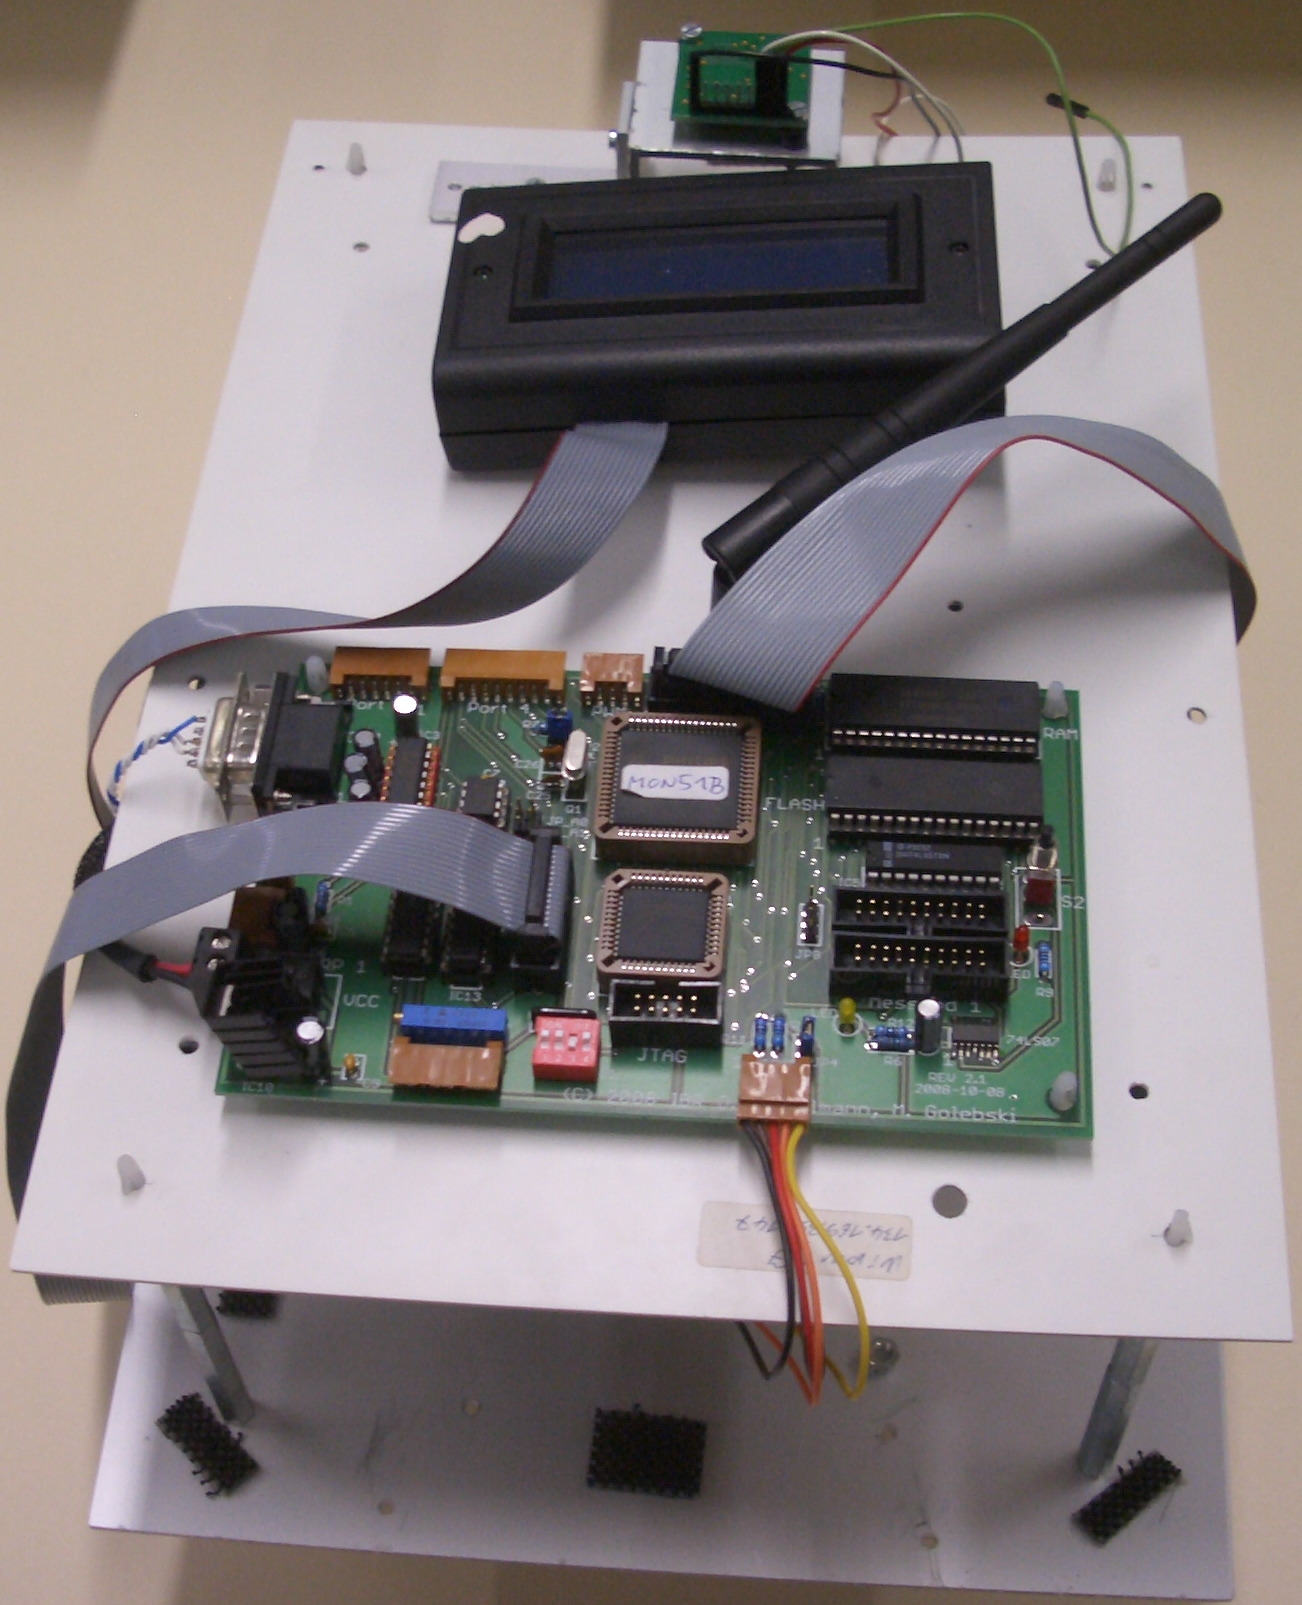
\includegraphics[width=0.48\textwidth]{pictures/fahrzeug.png}
	\end{multicols}
}

\frame{
	\begin{multicols}{2}
	\begin{itemize}
		\item Verbesserung des Protokolls
		\item Erweiterbarkeit
		\item Performanz
		\item Echtzeit-Aspekt
		\item Umfassende Dokumentation
	\end{itemize}
		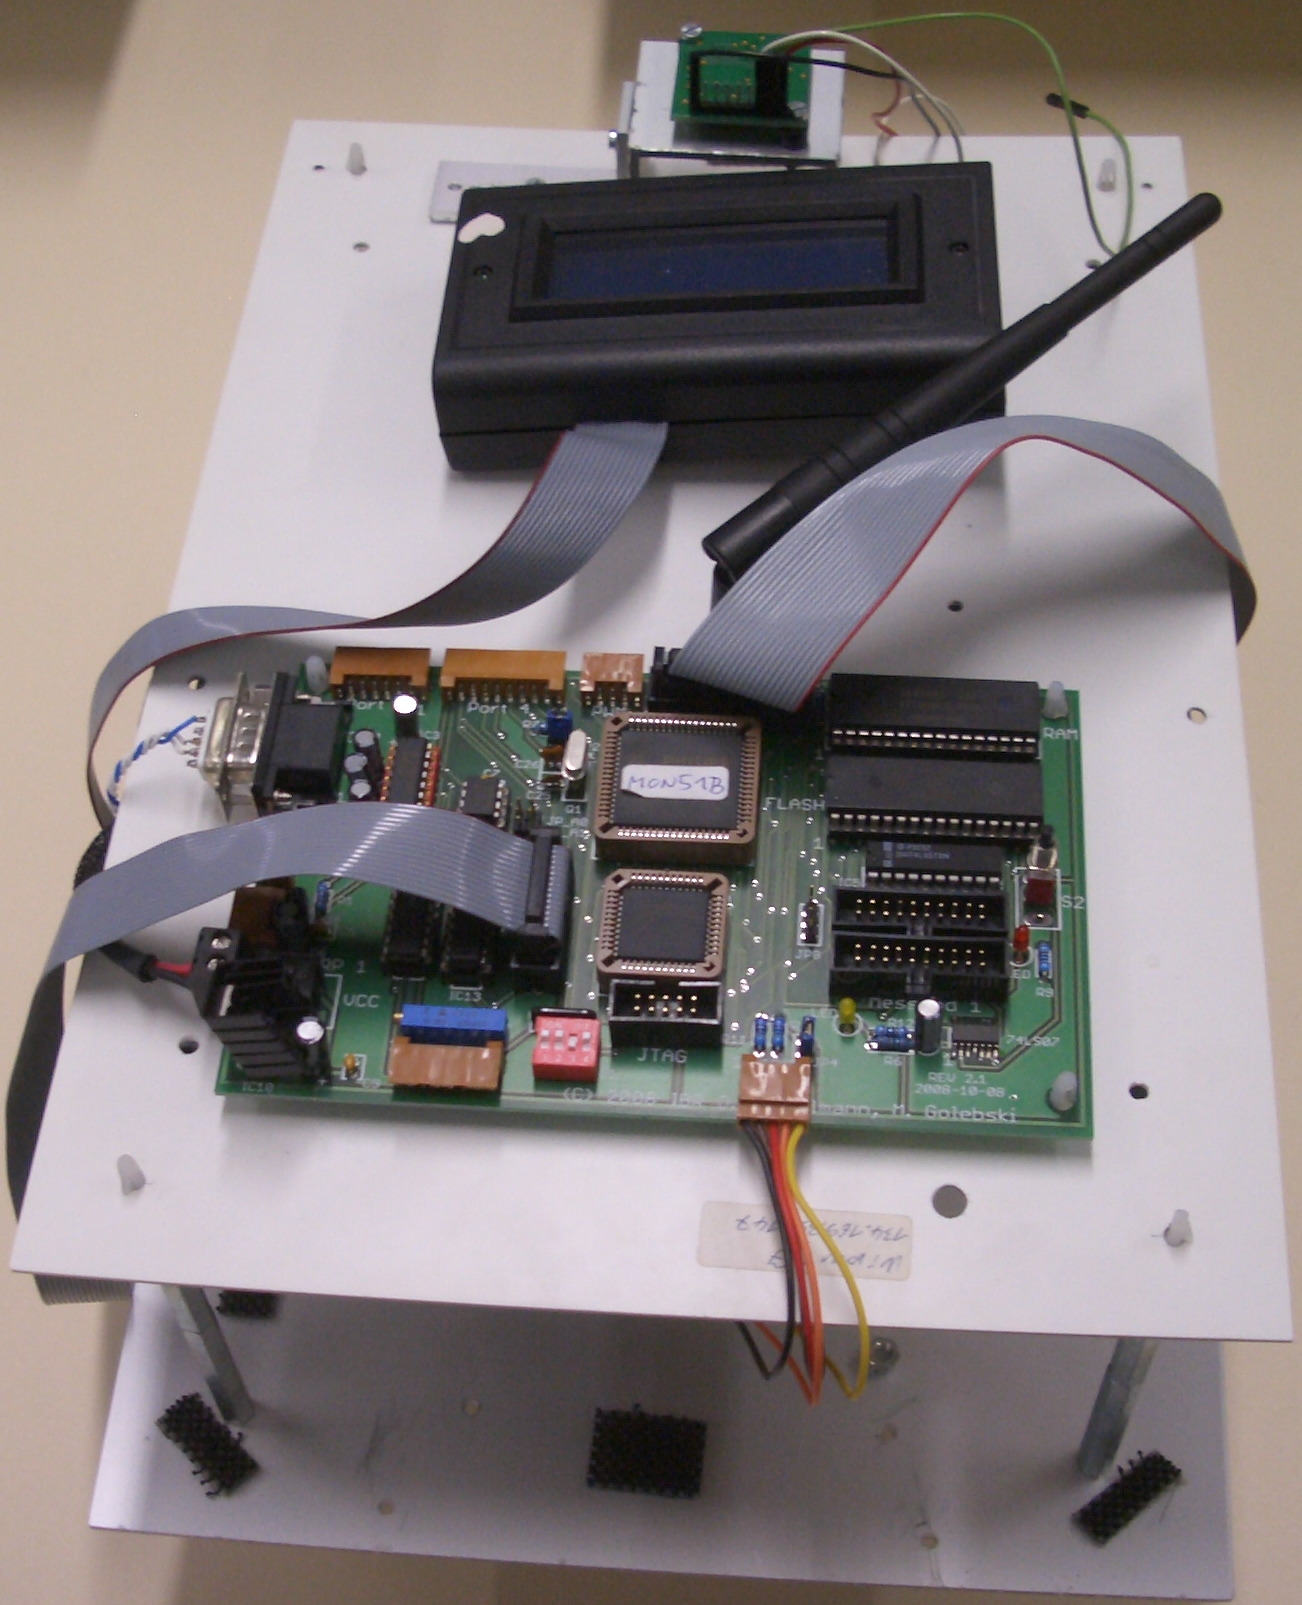
\includegraphics[width=0.48\textwidth]{pictures/fahrzeug.png}
	\end{multicols}
}

\section{Hardware}

\frame{
\frametitle{Die Motorplatine}
	\begin{itemize}
		\item AtMega 2561 (16 MHz, 8 KiB SRAM, 64 KiB Flash)
		\item PWM, I2C, UART, LCD
	\end{itemize}
\begin{figure}[h]
 \centering
 \scalebox{0.3}{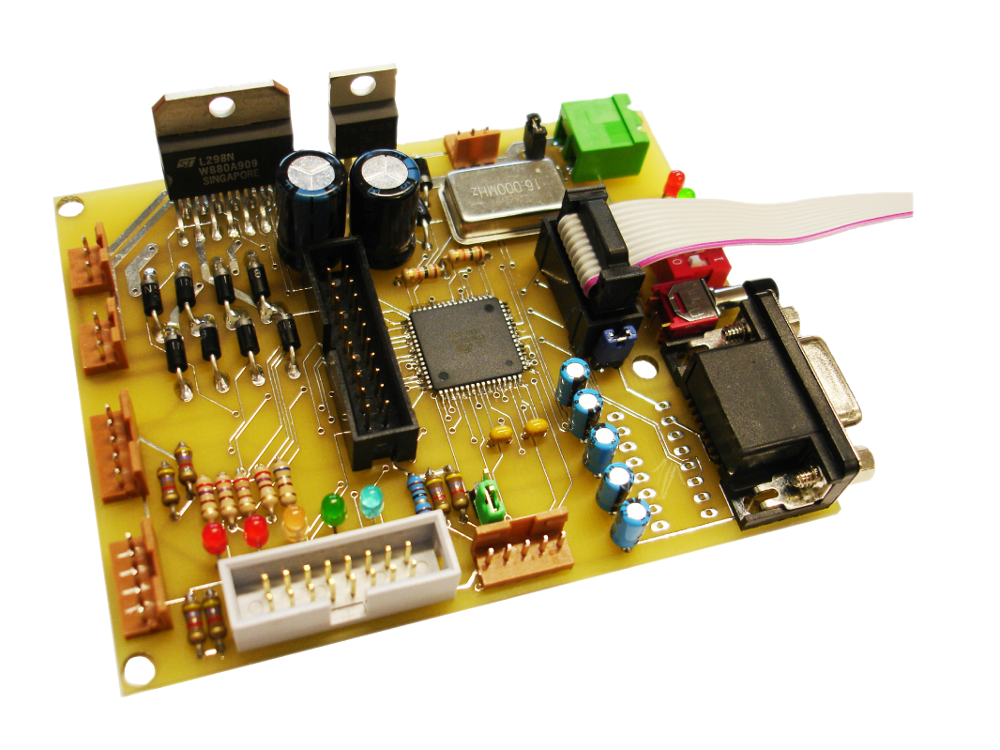
\includegraphics{pictures/motorplatine.png}}
\end{figure}
}

\frame{
\frametitle{Die Praktikumsplatine}
	\begin{itemize}
		\item Seite der Studierenden
		\item Anschluss an die Motorplatine über I2C
		\item Anschluss des WLAN-Moduls über UART
	\end{itemize}
\begin{figure}[h]
 \centering
 \scalebox{0.1}{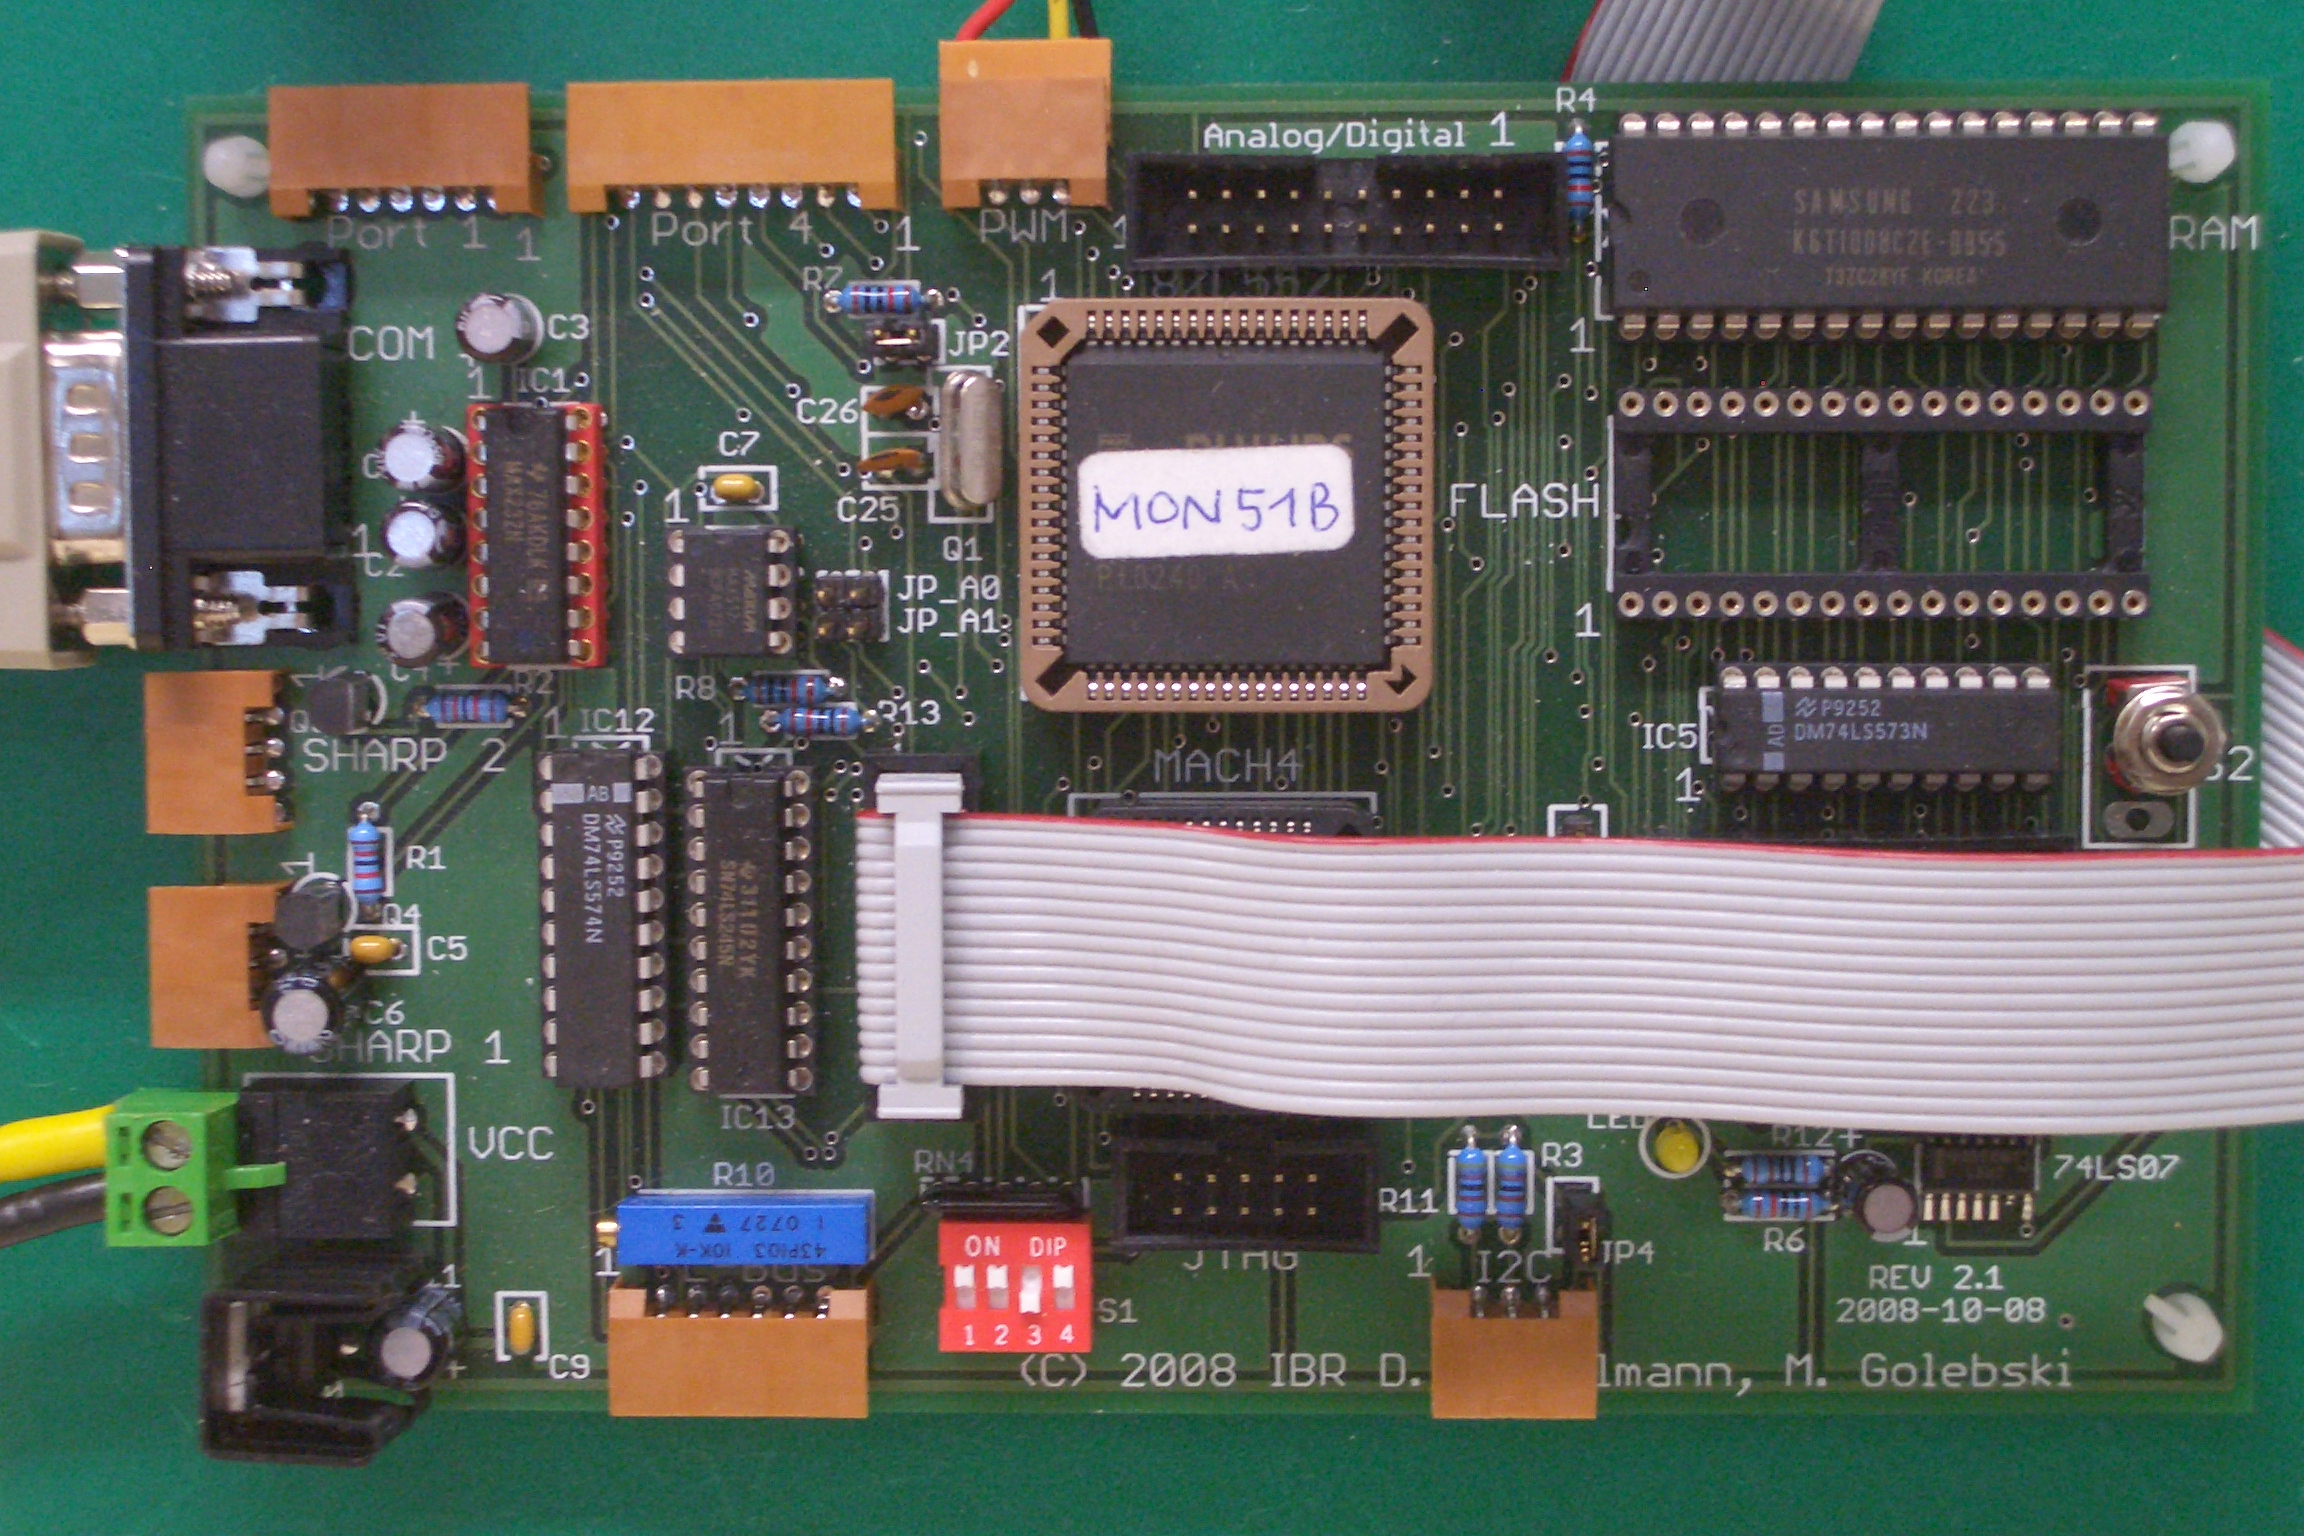
\includegraphics{pictures/praktikumsplatine.jpg}}
\end{figure}
}

\section{Design und Implementierung}

\frame{
\frametitle{Design-Prinzipien}
	\begin{itemize}
		\item Code in Module organisiert
		\item kurze, übersichtliche Funktionen
		\item generelle Funktionen
		\item wenige globale Variablen
		\item weniger inter-Modul Abhängigkeiten
	\end{itemize}
}

\frame{
\frametitle{Grundlegender Aufbau}
	\begin{itemize}
		\item Endlos-Schleife als Hauptschleife
		\item Periodisches Aktualisieren
	\end{itemize}
\begin{figure}[h]
 \centering
 \scalebox{0.5}{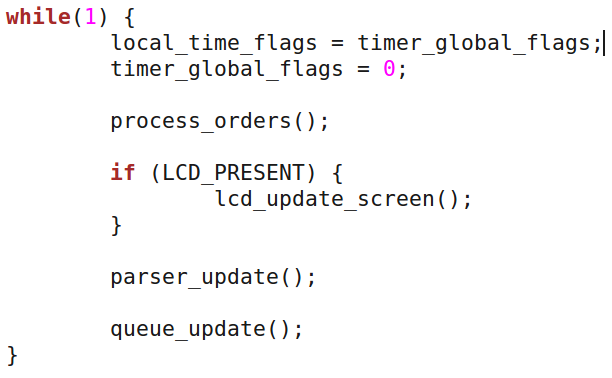
\includegraphics{pictures/main_loop_code.png}}
\end{figure}
}

\frame{
\frametitle{Protokoll}

\begin{figure}[h]
 \centering
 \scalebox{0.5}{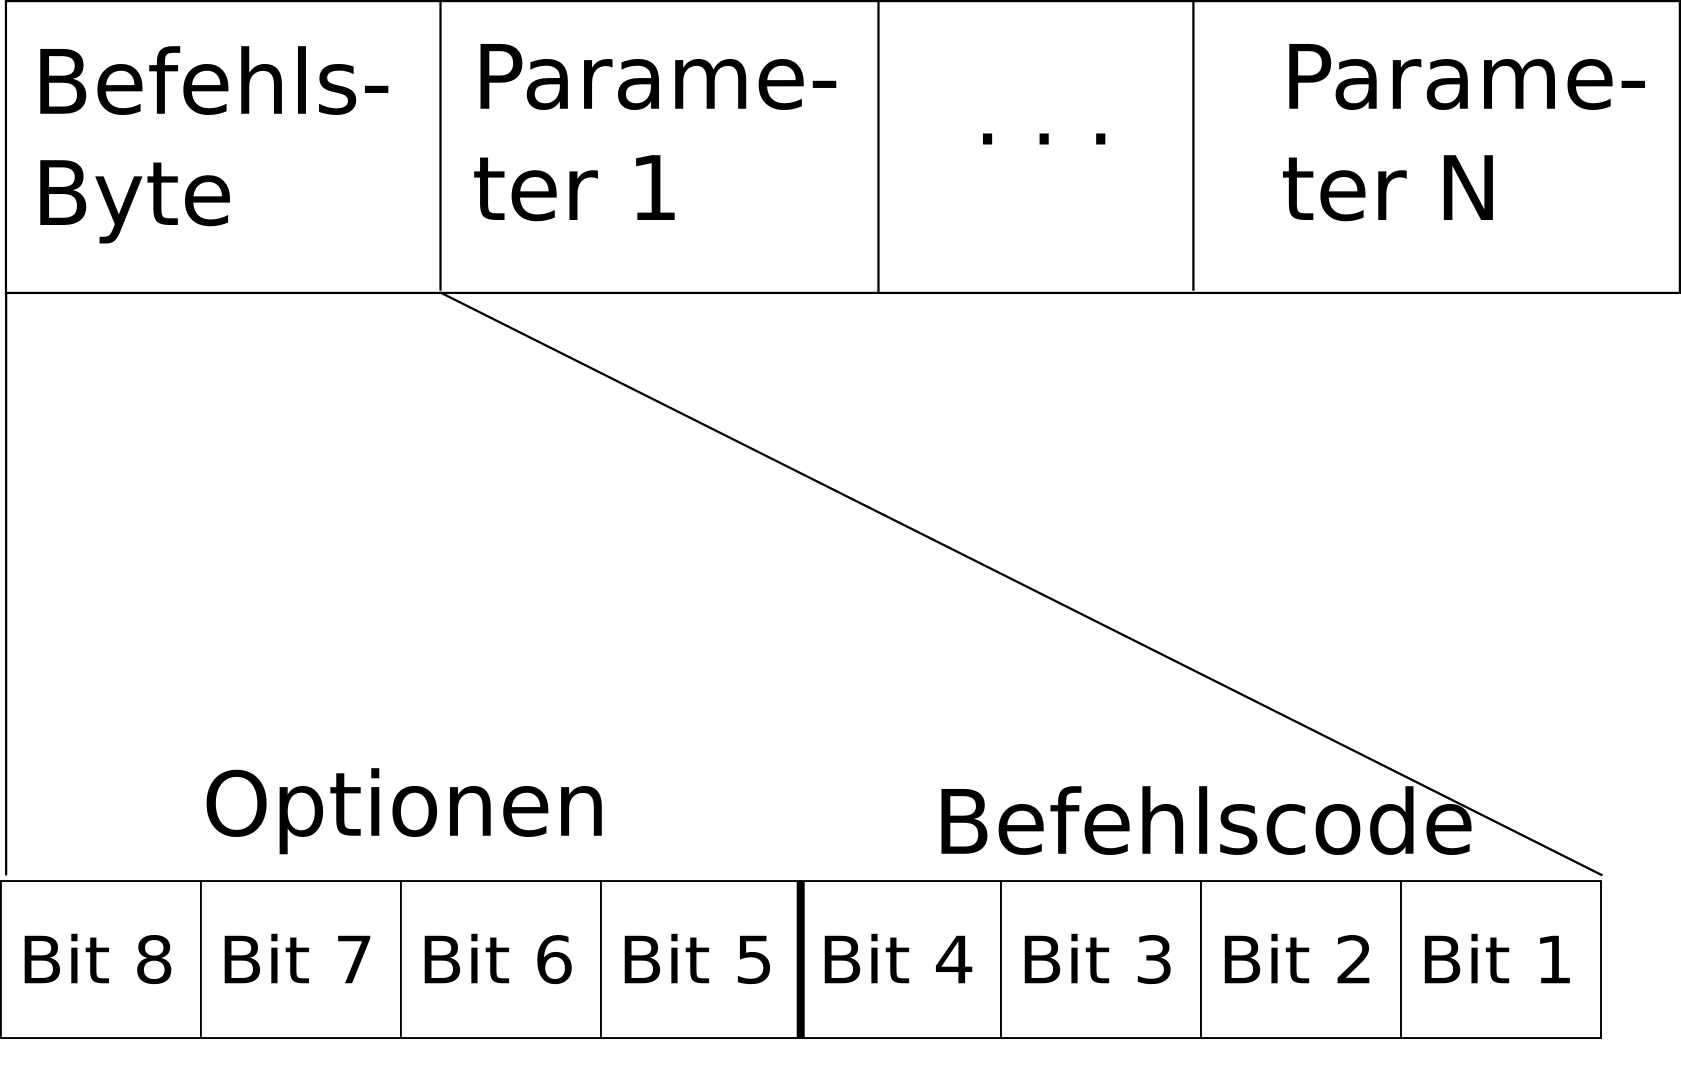
\includegraphics{pictures/protokoll.png}}
\end{figure}
}

\frame{
\frametitle{Die order\_t-Struktur}
	\begin{itemize}
		\item einfache Struktur
		\item flexibel Einsetzbar
		\item abstrakt, kein Wissen in der Struktur
	\end{itemize}
\begin{figure}[h]
 \centering
 \scalebox{0.4}{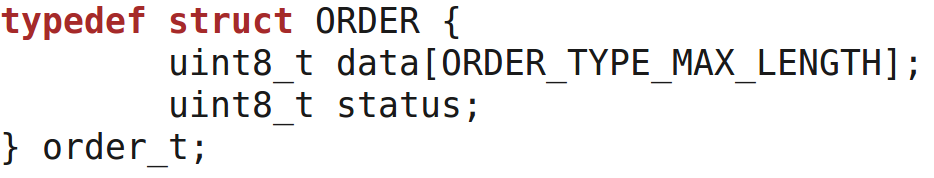
\includegraphics{pictures/order_t.png}}
\end{figure}
}

\frame{
\frametitle{Datenpfad der Befehle}
\begin{figure}[h]
 \centering
 \scalebox{0.6}{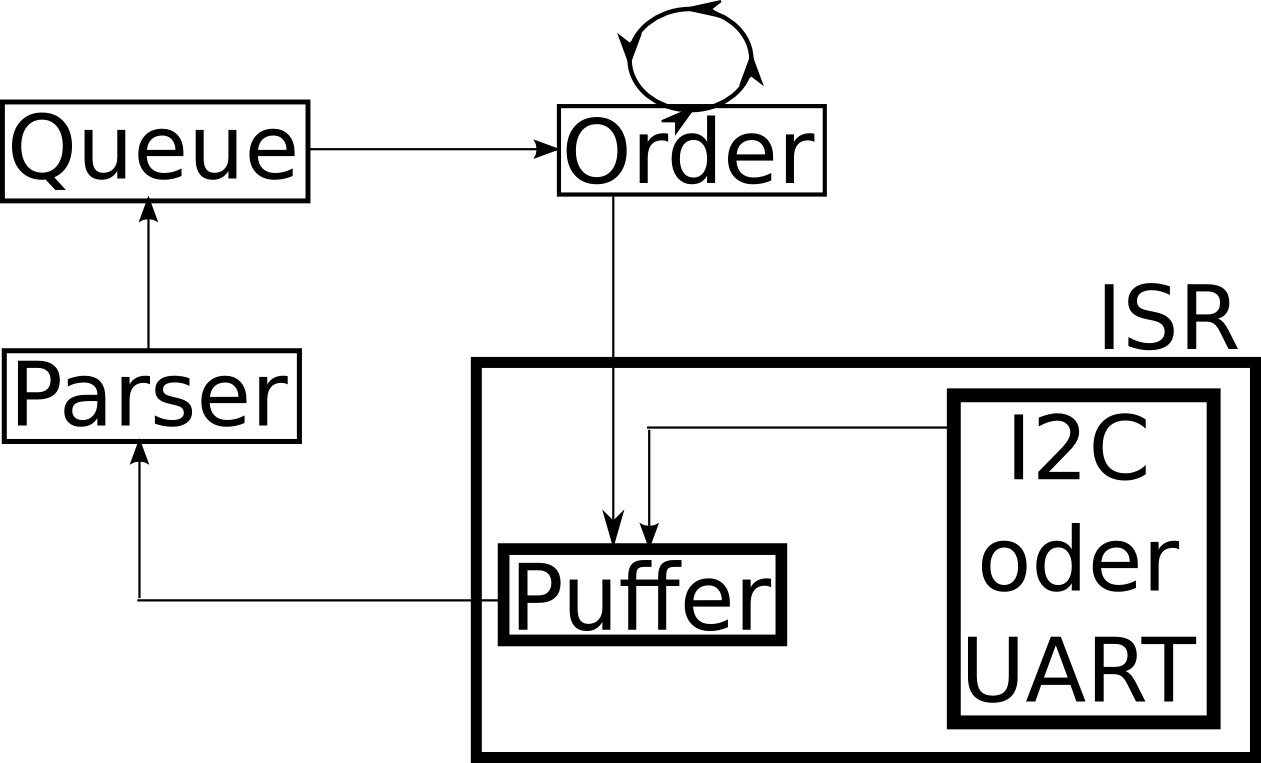
\includegraphics{pictures/pfad.png}}
\end{figure}
}

\frame{
	\centerline{Das Aktive-Brems-System}
	\begin{itemize}
		\item de-/aktivierbar und konfigurierbar
		\item Verhindert, dass sich das Fahrzeug ungewollt bewegt
	\end{itemize}
	\centerline{Das IO-Framework}
	\begin{itemize}
		\item abstrahiert die Ein-/Ausgabe über UART und I2C
		\item es werden die selben Funktionen benutzt
	\end{itemize}
}

\frame{
\frametitle{Bibliothek}
	\begin{itemize}
		\item Praktikumsplatine muss mit der Motorplatine kommunizieren
		\item Befehle erstellen
		\item Befehle direkt senden
	\end{itemize}
\begin{figure}[h]
 \centering
 \scalebox{0.3}{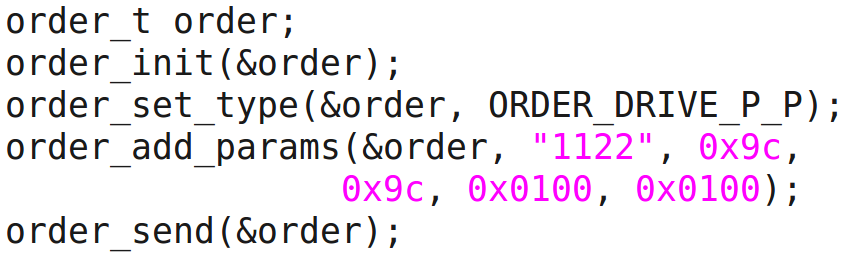
\includegraphics{pictures/bibliothek.png}}
\end{figure}
}

\section{Untersuchung}

\frame{
\frametitle{Untersuchung}
	\begin{itemize}
		\item Pins setzen/zurücksetzen (Makros)
		\item auslesen mit Logik-Analyser
		\item pin\_set() und pin\_clear() benötigen 250 ns
		\item pin\_toggle() benötigt 250 ns
	\end{itemize}
\begin{figure}[h]
 \centering
 \scalebox{0.29}{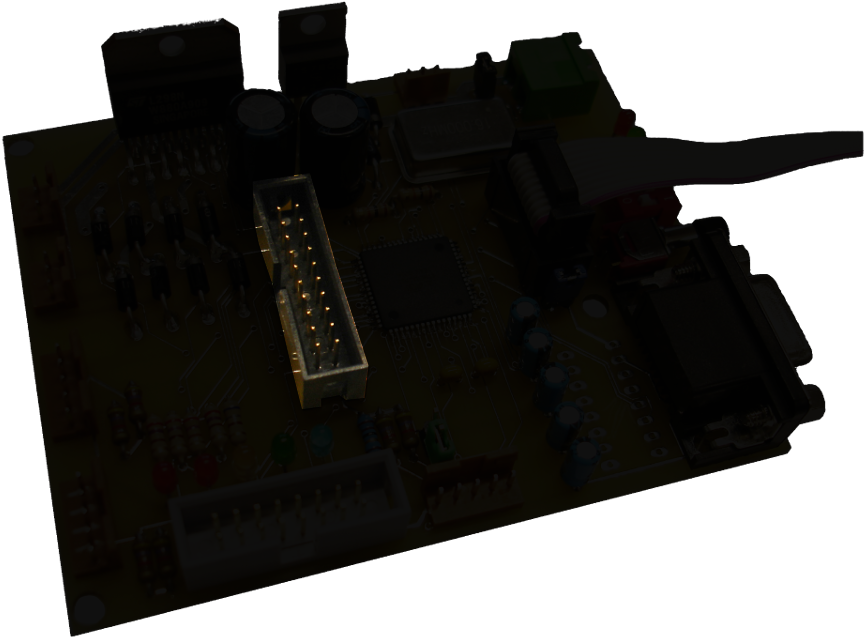
\includegraphics{pictures/motorplatine_mod.png}}
\end{figure}
}

\frame{
\frametitle{Verzögerungs-Problem}
\begin{figure}[h]
 \centering
 \scalebox{0.3}{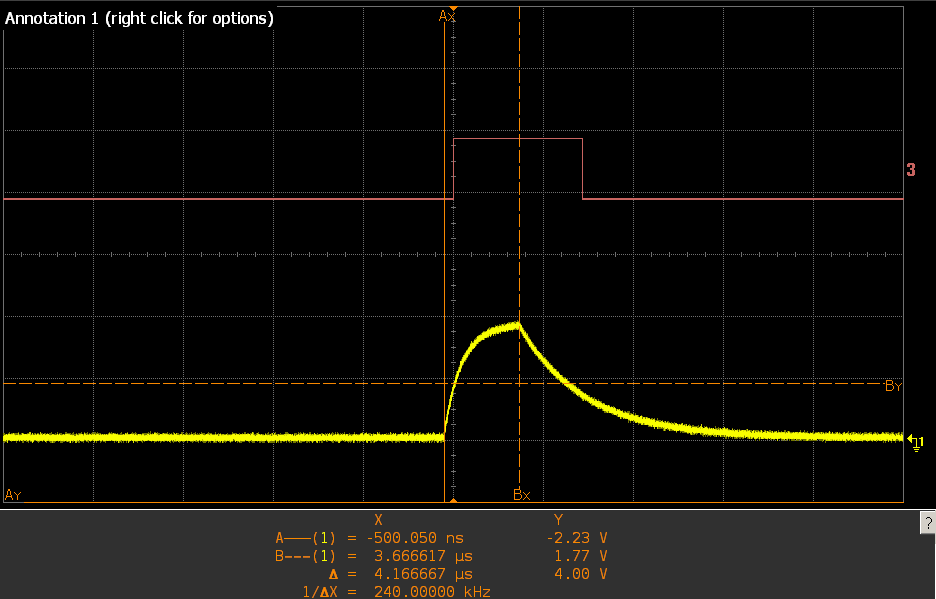
\includegraphics{pictures/messbild.png}}
\end{figure}
}

\frame{
\frametitle{LCD-Problem}
	Vorher:
	\begin{itemize}
		\item Busy-Waiting benötigt 3250 us
		\item Ein Aufruf
		\item Merkbare Latenz
	\end{itemize}
	Nachher:
	\begin{itemize}
		\item max. 1 Zeichen pro Iteration benötigt 60 us
		\item Dauernder Aufruf, während noch Daten zu aktualisieren sind
		\item leicht erhöhte Idle-Zeit
		\item zusätzlicher Speicher für Puffer
	\end{itemize}
}

\frame{
\centerline{Compiler-Optimierung}
	\begin{itemize}
		\item Wechsel von -Os auf -O2
		\item Inlining von Funktionen (ca. 32\% Verbesserung)
	\end{itemize}
\centerline{Modulo-Operatoren}
	\begin{itemize}
		\item Benötigen viel Zeit (ca. 13 us pro \%)
		\item Einfach zu ersetzen mithilfe von -, / und *
		\item Verbraucht dann bis zu 90\% weniger Zeit
	\end{itemize}
}

\frame{
\frametitle{Echtzeit}
	\begin{itemize}
		\item Ist es möglich Interrupts zu verpassen/verlieren?
		\item Nein. Interrupts werden zwischengespeichert und später ausgeführt.
		\item Worst Case: 8 Ints * 10 us = 80 us (schnellster Int tritt alle 138 us auf)
	\end{itemize}
}

\frame{
\frametitle{Vergleich}
\begin{table}[htb]
\begin{center}
	\small
	\begin{tabular}{|l||c|}
		\hline
		\textbf{Funktion} & \textbf{Zeit} \\ \hline \hline
		Hauptschleife (Vorläufer) & 121,885 \textmu{}s \\ \hline
		Hauptschleife (aktuell) & 23,535 \textmu{}s \\ \hline \hline
		Befehl (kurz, Vorläufer) & 3655 \textmu{}s (13 Byte) \\ \hline
		Befehl (kurz, aktuell) & 1023 \textmu{}s ( 4 Byte) \\ \hline
		Befehl (lang, Vorläufer) & 7747 \textmu{}s (27 Byte) \\ \hline
		Befehl (lang, aktuell) & 2191 \textmu{}s ( 8 Byte) \\ \hline
	\end{tabular}
\end{center}
\end{table}
}

\section{Fazit}
 
\frame{
\frametitle{Ziele erreicht}
	\begin{itemize}
		\item gleiche Funktionalität
		\item Erweiterbar
		\item schneller als Vorläufer
		\item Protokoll neu implementiert
	\end{itemize}
}

\frame{
\frametitle{Ideen für die Zukunft}
	\begin{itemize}
		\item bessere Fehlererkennung des Parsers
		\item erhöhte Robustheit durch einen Sanity-Checker
		\item Verwendung der Energie-Spar-Funktionen
	\end{itemize}
}

\end{document}
